\documentclass[10pt]{article}
\usepackage[margin=1.5cm]{geometry}
\usepackage{lmodern}
\usepackage[T1]{fontenc}
\usepackage[utf8]{inputenc}
\usepackage[french]{babel}
\usepackage[absolute]{textpos}
\usepackage[usenames,dvipsnames]{color}
\usepackage{array}
\usepackage{titlesec}
\usepackage{graphicx}
\usepackage{hyperref}

\definecolor{lightgray}{gray}{0.8}
\definecolor{darkgray}{gray}{0.35}
\newcolumntype{L}{>{\raggedleft}p{0.14\textwidth}}
\newcolumntype{R}{p{0.8\textwidth}}
\newcommand\VRule{\color{lightgray}\vrule width 0.5pt}
\newcommand{\emphcolor}{NavyBlue}
\newcommand{\cemph}[1]{{\color{\emphcolor} #1}}
\titleformat{\section}{\color{\emphcolor}\normalfont\Large\bfseries}{\thesection}{1em}{}[{\titlerule[0.2pt]}]

\hypersetup{colorlinks=true, urlcolor=\emphcolor}

\begin{document}
\thispagestyle{empty}
%%%%%%%%%%%%%%%%%%%%%%%%%%%%%%%%%%%%%%%%%%%%%%%%%%%%%%%%%%%%%%%%%%%%%%%%%%%%%%%%
%	HEADER

% Informations personnelles
\begin{textblock}{7}(0.2,0.4)
	\begin{tabular}{l}
		\small
		Hameau Les Vaux,\\ 77370 Rampillon\\
		26 ans (1987-04-24)\\
		tél. : 06 87 63 83 13\\
		mél. : \texttt{yankel.scialom@mail.com}\\
		Permis B
	\end{tabular}
\end{textblock}

% Name
\begin{textblock}{7}(7.5,1.2)
	{\Huge Yankel \textsc{Scialom}}
	
	\vspace{1em}\hspace{3em}{\large\color{darkgray}\textit{Ingénieur informatique junior}}
\end{textblock}

% Photo
\begin{textblock}{7}(12.9,0.4)
	{\color{\emphcolor}\fbox{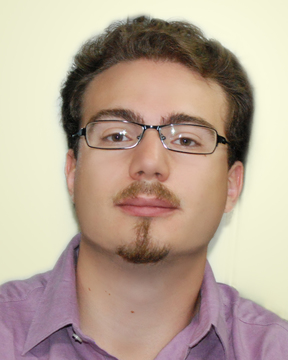
\includegraphics{photo-min}}}
\end{textblock}

% Destinataire
% YAPA

% Accroche
\begin{textblock}{16}(0,2.55)
	\centering
	\fontsize{15pt}{18pt}\selectfont
	\cemph{\textsc{Jeune ingénieur passionné, cherche emploi développement informatique}}
\end{textblock}

%%%%%%%%%%%%%%%%%%%%%%%%%%%%%%%%%%%%%%%%%%%%%%%%%%%%%%%%%%%%%%%%%%%%%%%%%%%%%%%%
%	BODY

\fontsize{10pt}{10pt}\selectfont
\begin{textblock}{14}(0.5,2.8)

% jobs
	\section*{Expériences professionnelles}
	\begin{tabular}{L!{\VRule}R}
	%
	2013--présent&{\bf Auto-formation, projets divers, voyages}\\
	& \begin{itemize}
		\item Sécurité informatique et \textit{pentests}, mathématiques pour l'ingénieur,
	protocoles réseau, administration système~(linux), outils de gestion de projet, divers.
		\item Logiciel opensource \href	{https://github.com/yoannsculo/JobCatcher}{JobCatcher},
			\textit{Pentest box} Android, serveur SMS embarqué, agent de notification
			pour \textit{desktop} gnome.
		\item Londres, Oxford, Canterbury (RU) ; Bavière (Allemagne) ; Belgrade, Ra\v{c}a (Serbie) ;
			France (nombreuses villes) ; Barcelone (Espagne) ; Vietnam (circuit touristique).
	\end{itemize}\\
	
	%
	2012 & {\bf \textsc{Sysnav}, stage de fin d'études}\\
	& Conception \& développement, test \& documentation d'un système d'exploitation
	temps-réel pour micro-contrôleur \textsc{Renesas}.\\
	
	%
	\rule{0pt}{3ex}2010 & {\bf \textsc{Thales Optronique} S.A., stage professionel}\\
	& Développement d’une interface homme-machine pour une suite logicielle de
	gestion de drones aériens.\\
	
	%
	\rule{0pt}{3ex}Juillet 2008 & {\bf \textsc{Battenfeld} France S.A.S.}\\
	& Traduction Allemand/Anglais/Français de documentations techniques de presses hydroliques ;\\
	& étude de fonctionnalités réseau d’un système embarqué Windows.\\
	
	%
	\rule{0pt}{3ex}2005--2012 & {\bf Cours particuliers et divers jobs d'été}\\
	& Cours de remise à niveau et préparation au Baccalauréat en mathématiques,
	physique-chimie et biologie ;\\
	& caissier, magasinier, vendeur, etc.
	\end{tabular}

% studies
	\section*{Formation}
	\begin{tabular}{L!{\VRule}R}
	%
	2012 & {\bf Université de technologies de Troyes}\\
	& Obtention du diplôme d'ingénieur en systèmes d'informations et télécommunication,
	spécialité technologies mobiles et systèmes embarqués, mineur gestion d'entreprise.\\
	
	%
	\rule{0pt}{3ex}2010 & {\bf \textsc{Bullats}}\\
	& Obtention du diplôme de langue, niveau européen B2 en anglais.\\
	
	%
	\rule{0pt}{3ex}2008 & Validation de la première année du cycle d'ingénieur en systèmes mécaniques.\\
	
	%
	\rule{0pt}{3ex}2005 & {\bf Baccalauréat Scientifique}\\
	& spécialité mathématiques, obtention avec mention.
	\end{tabular}

% misc.
	\section*{Divers}
	\begin{tabular}{L!{\VRule}R}
	%
	& {\bf Connaissances technologiques}\\
	& \begin{itemize}
		\item Langages de développement :  C/C++ (Qt, Boost), Java EE (Servlet, EJB,
	JDBC, ...), Web (Linux, Apache, [My|Psotgre]SQL, PHP, HTML, CSS, Javascript,
	jQuery[-ui], ...).
		\item Outils et langages liés aux technologies embarqués : ASM, VHDL,
	Java pour Android, noyau linux, fonctionnement d'un ALU, etc..
		\item Divers outils et langages généraux : OCaml, Lisp, ActionScript,
	VirtualBasic, python, bash, \textit{versionning} (git, svn, trac), suivis de bugs,
	réseaux, administration système, etc..
	\end{itemize}\\
	
	%
	\rule{0pt}{3ex} & {\bf Langues}\\
	& Français (langue maternelle), Anglais (couramment lu/compris, bien écris/parlé ;
	niveau B2 validé en 2010), Allemand (notions), Serbo-croate (en cours d'apprentissage).\\
	
	%
	\rule{0pt}{3ex} & {\bf Loisirs}\\
	& Passionné de technologies ; photographe amateur ; cinéphile.
	\end{tabular}
\end{textblock}
\end{document}
